\documentclass[a4paper, 12pt]{article}%тип документа

%отступы
\usepackage[left=2cm,right=2cm,top=2cm,bottom=3cm,bindingoffset=0cm]{geometry}

%Русский язык
\usepackage[T2A]{fontenc} %кодировка
\usepackage[utf8]{inputenc} %кодировка исходного кода
\usepackage[english,russian]{babel} %локализация и переносы

%Вставка картинок
\usepackage{wrapfig}
\usepackage{graphicx}
\graphicspath{{pictures/}}
\DeclareGraphicsExtensions{.pdf,.png,.jpg}

%оглавление
\usepackage{titlesec}
\titlespacing{\chapter}{0pt}{-30pt}{12pt}
\titlespacing{\section}{\parindent}{5mm}{5mm}
\titlespacing{\subsection}{\parindent}{5mm}{5mm}
\usepackage{setspace}

%Графики
\usepackage{multirow}
\usepackage{pgfplots}
\pgfplotsset{compat=1.9}

%Математика
\usepackage{amsmath, amsfonts, amssymb, amsthm, mathtools}

%Заголовок
\author{Валеев Рауф Раушанович \\
группа 825}
\title{\textbf{Работа 3.3.5\\
Эффект Холла в металлах}}
\begin{document}
\maketitle
\newpage
\section*{Цель работы.}
Измерение подвижности и концентрации носителей заряда в металлах.\\
\section*{В работе используются.}
Электромагнит с источником питания, источник постоянного тока, микровольтметр, амперметры, милливеберметр, образцы из меди и цинка. 
\section*{Теоретическая справка.}
Суть эффекта Холла состоит в следующем. Пусть через однородную пластину металла вдоль оси $x$ течёт ток $I$\\
Если эту пластину поместить в магнитное поле, направленное по оси $y$, то между гранями А и Б появляется разность потенциалов. В самом деле, на электрон, движущийся со скоростью $<v>$ в электромагнитном поле, действует сила Лоренца: 
\begin{equation}
F_l = -eE - e<v> \times B
\end{equation}
где, $e$ - абсолютная величина заряда электрона, $E$ - напряженность электрического поля, $B$ - индукция магнитного поля. 
В нашем случае сила, обусловленная вторым слагаемым, направлена вдоль оси $z$
\[F_B = e |<v_x>|B\]
Под действием этой силы электроны отклоняются к грани Б, заряжая её отрицательно (для простоты рассматриваем только один тип носителей). На грани А накапливаются нескомпенсированные положительные заряды. Это приводит к возникновению электрического поля $E_z$, направленного от А к Б, которое действует на электроны с силой $F_E = e E_z$, направленной против силы $F_B$. В установившемся режиме сила $F_E$ уравновешивает силу $F_B$, и накопление электрических зарядов на боковых гранях пластины прекращается.\\
Из условия $F_B = F_E$ найдем 
\begin{equation}
E_z = |<v_x>|B
\end{equation}
Поле $E_z$ дает вклад в общее поле $E$, в котором движутся электроны. С полем $E_z$ связано разность потенциалов $U_{\text{АБ}}$ между гранями A и Б
\begin{equation}
U_{\text{АБ}} = -E_z l = -|<v_x>|Bl
\end{equation}
В этом и состоит эффект Холла. Второе слагаемое в силе Лоренца, с которым связан эффект, называют "холловским".
\begin{equation}
I = ne|<v_x>|l \cdot a 
\end{equation}
\begin{equation}
\varepsilon_x = U_{\text{АБ}} = -\dfrac{IB}{nea} = -R_x \cdot \dfrac{IB}{a}
\end{equation}
Константа $R_x$ называется постоянной Холла. Как видно, она равна \begin{equation}
R_x = \dfrac{1}{ne}
\end{equation}
\section*{Экспериментальная установка.}
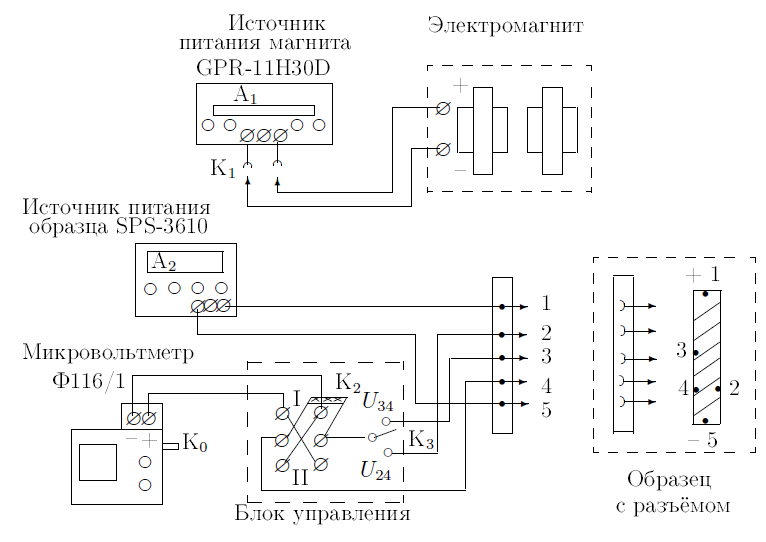
\includegraphics[width = \textwidth]{5.png}\\
\begin{center}
\textbf{Рисунок 1.}Схема установки для исследования эффекта Холла в металлах.
\end{center}
В зазоре электромагнита создается постоянное магнитное поле, которое можно регулировать с помощью источника питания электромагнита.\\
Иногда контакты 2 и 4 вследствие неточности подпайки не лежат на одной эквипотенциали, и тогда напряжение между ними связано не только с эффектом Холла, но и с омическим напряжением, вызванным протеканием основного тока через образец. \\
Неточности измерений можно избежать путем фиксирования этого омического напряжения при нулевом значении силы тока и отсчитывании от него Холловского напряжения. 
\[\varepsilon_x = U_{24} \pm U_0\]
Измерив ток в образце и нарпяжение $U_{34}$ между контактами 3 и 4 в отсутствии магнитного поля, можно, зная параметры образца, рассчитать проводимость материала образца по очевидной формуле:
\begin{equation}
\sigma = \dfrac{I L_{34}}{U_{34}al}
\end{equation}

\section*{Ход работы.}
Проводим измерение зависимости магнитного потока от величины силы тока. Результаты приведены в таблице и на графике ниже.\\
\begin{center}
\begin{tabular}{|c|c|c|c|c|}
\hline
 & $I_{\text{м}}, A$ & $\sigma_{I_{\text{м}}}, A$ & $B, \text{мТл}$ & $\sigma_{B}, \text{мТл}$ \\ \hline
1 & 0,20 & 0,01 & 230 & 10 \\ \hline
2 & 0,35 & 0,01 & 400 & 20 \\ \hline
3 & 0,50 & 0,01 & 580 & 30 \\ \hline
4 & 0,65 & 0,01 & 780 & 40 \\ \hline
5 & 0,80 & 0,01 & 930 & 50 \\ \hline
6 & 0,96 & 0,01 & 1050 & 55 \\ \hline
\end{tabular}\\
\textbf{Таблица 1.}$B = f(I_{\text{м}})$

\end{center}
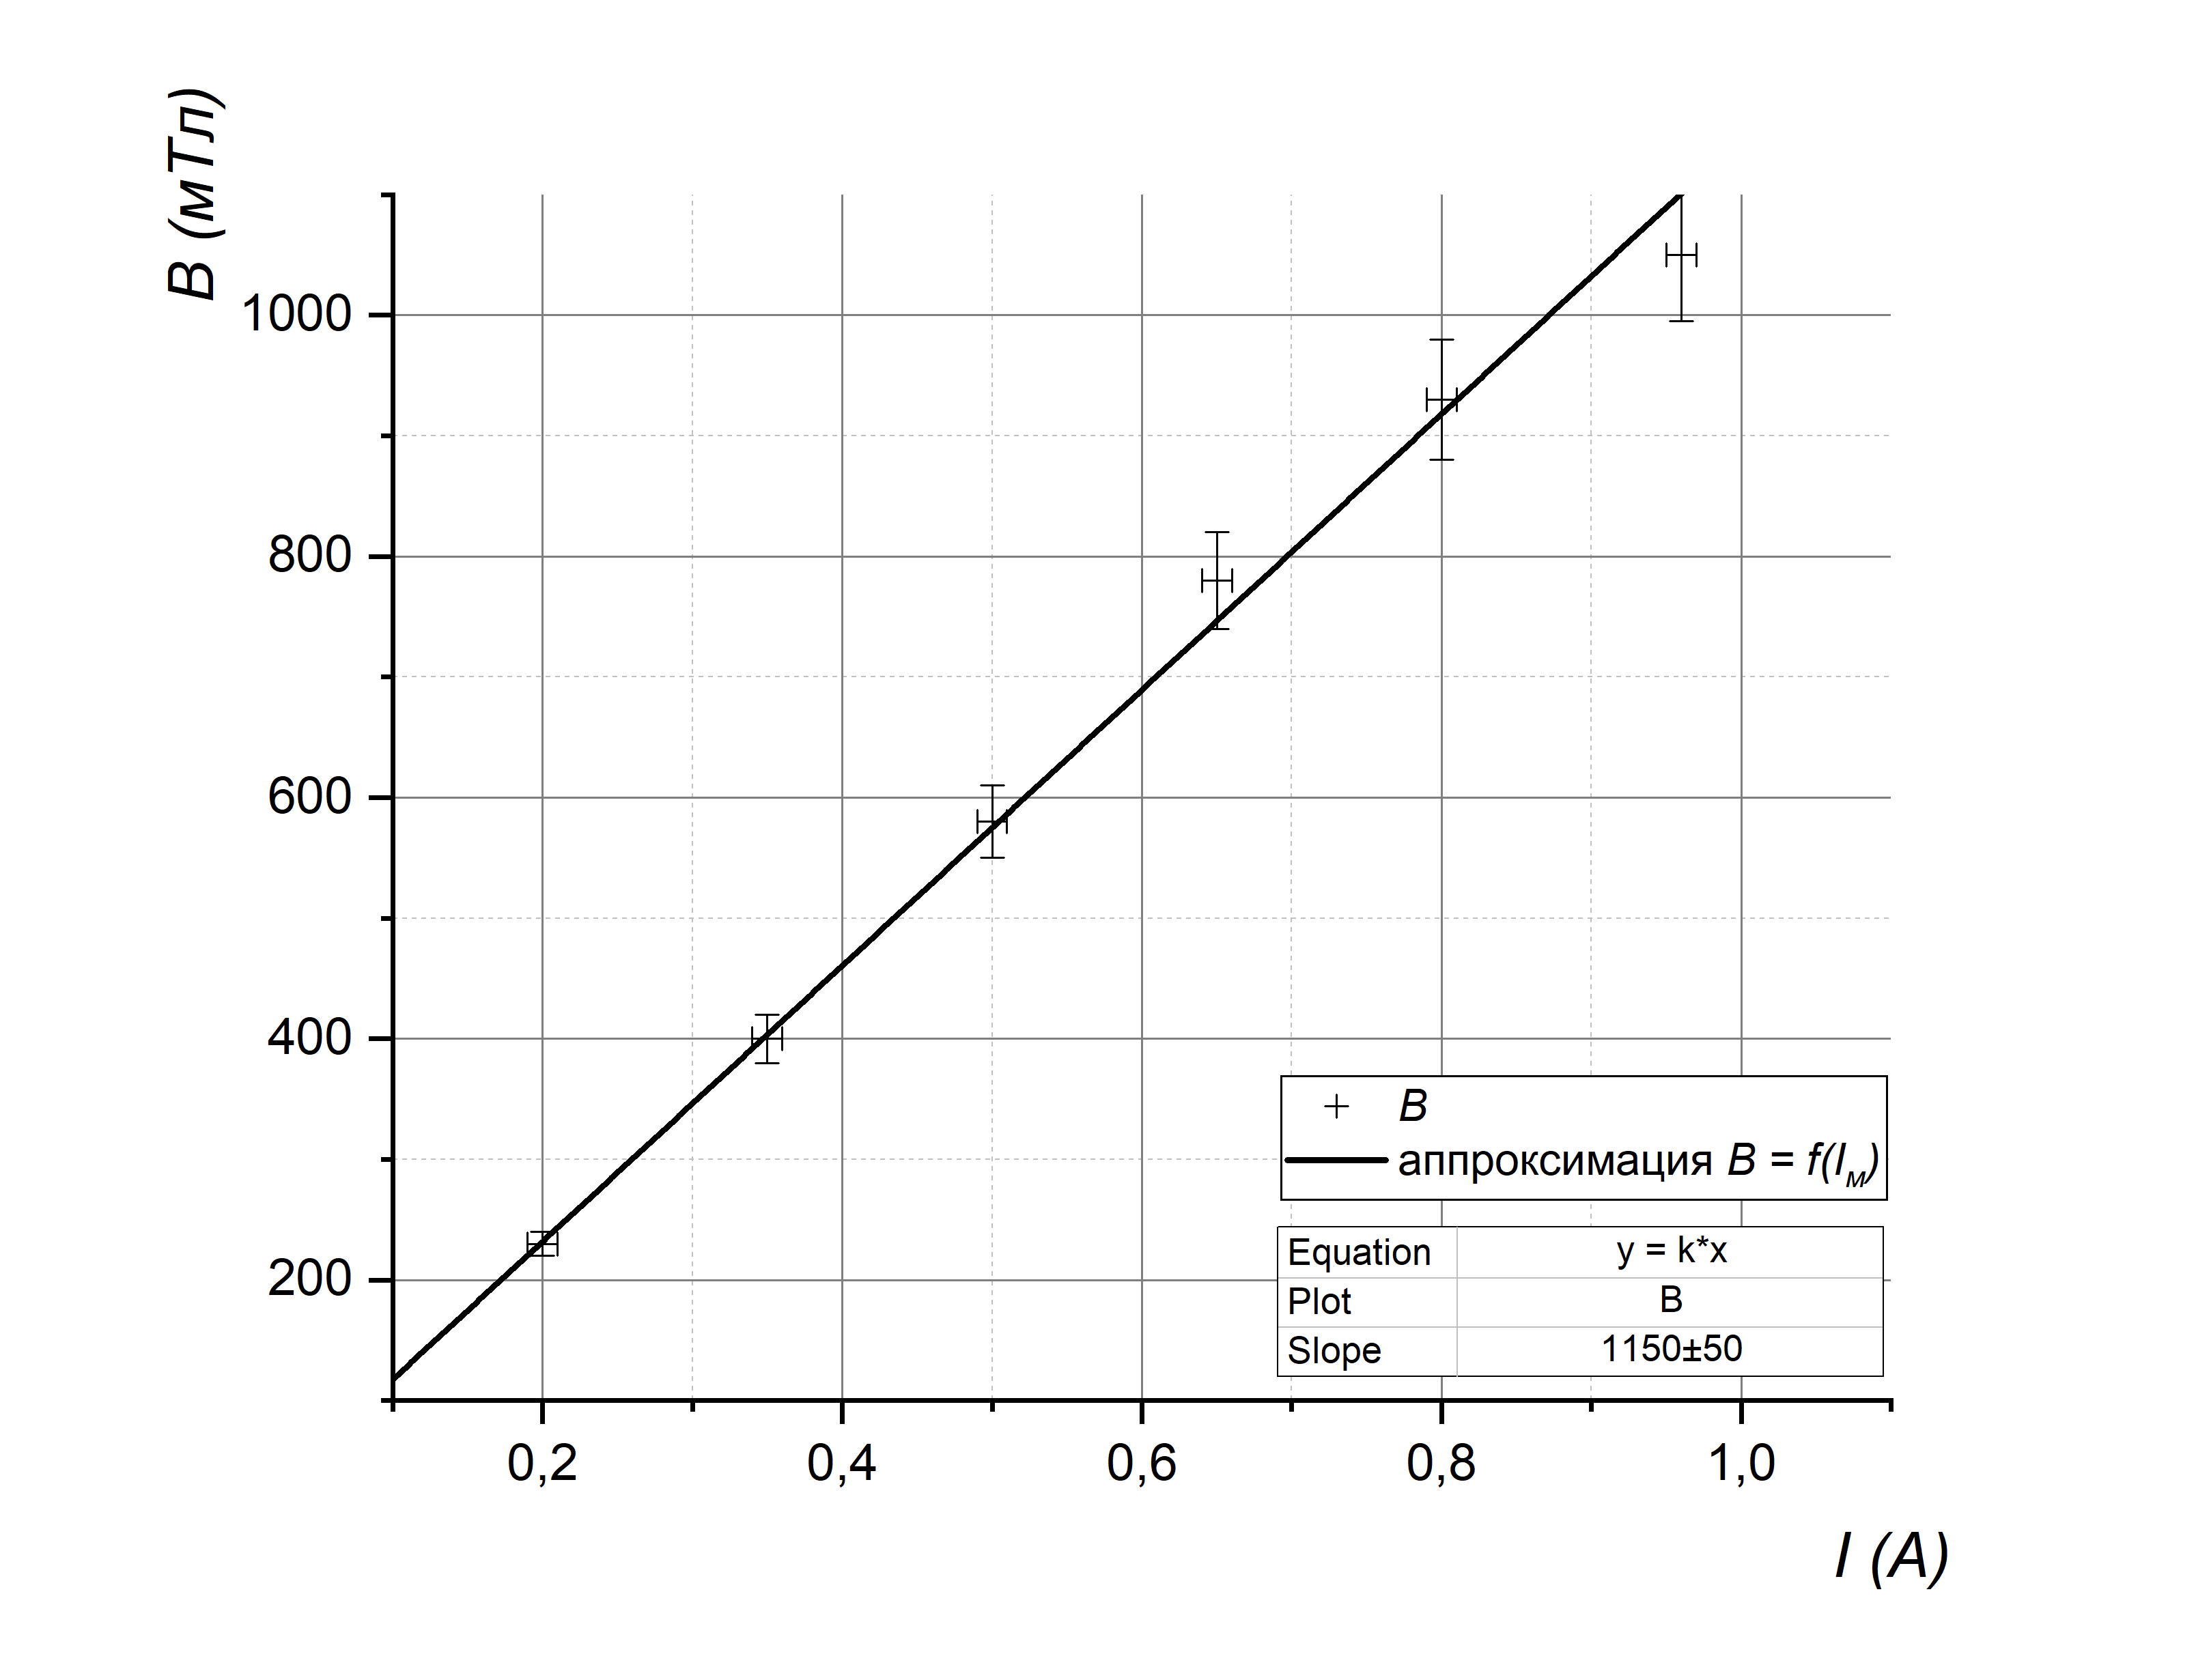
\includegraphics[width = \textwidth]{1.jpg}
\begin{center}
\textbf{График 1.}Нахождение $B = f(I_{\text{м}}$)
\end{center}

Проводим измерения ЭДС Холла. Для этого вставляем образец в зазор выключенного электромагнита и определяем $U_0$ между контактами 2 и 4. Это значение следует принять за 0. \\
Далее включаем электромагнит и измеряем $U = f(I_{\text{м}}$ для образца из меди.
\\
Проводим серию для 5 значений тока через образец.\\
То же делаем для образца из цинка при одном фиксированном значении тока через образец.\\
Определяем знак носителей заряда для каждого из материалов. \\
Для цинка получается -.\\
Для меди - +.\\
\begin{center}
\begin{tabular}{|c|c|c|c|c|c|c|c|}
\hline
 & \multicolumn{3}{c|}{$(I = 0,4 \pm 0,01)$ А} & \multicolumn{4}{c|}{$U_0 = (2 \pm 1)$ ед.} \\ \hline
 & $I_{\text{м}}$, А & $\sigma_{I_{\text{м}}}, A$ & $\sigma_B$, мТл & $B$, мТл & $U$, ед & $U$, нВ & $\sigma_{U}$, нВ \\ \hline
1 & 0,20 & 0,01 & 130 & 230 & 3 & 40 & 20 \\ \hline
2 & 0,39 & 0,01 & 80 & 450 & 5 & 120 & 20 \\ \hline
3 & 0,60 & 0,01 & 70 & 700 & 7 & 200 & 20 \\ \hline
4 & 0,80 & 0,01 & 65 & 900 & 9 & 280 & 20 \\ \hline
5 & 1,01 & 0,01 & 70 & 1150 & 10 & 320 & 20 \\ \hline
6 & 1,20 & 0,01 & 80 & 1400 & 11 & 360 & 20 \\ \hline
\end{tabular}\\
\textbf{Таблица 2:} Для тока через материал $I = 0,4$ A\\
\begin{tabular}{|c|c|c|c|c|c|c|c|}
\hline
 & \multicolumn{3}{c|}{$(I = 0,6 \pm 0,01)$, А} & \multicolumn{4}{c|}{$U_0 = (3 \pm 1)$ ед.} \\ \hline
 & $I_{\text{м}}$, А & $\sigma_{I_{\text{м}}}, A$ & $B$, мТл & $\sigma_B$,мТл & $U$, ед & $U$, нВ & $\sigma_{U}$, нВ \\ \hline
1 & 0,20 & 0,01 & 230 & 90 & 8 & 240 & 20 \\ \hline
2 & 0,40 & 0,01 & 450 & 80 & 12 & 400 & 20 \\ \hline
3 & 0,60 & 0,01 & 700 & 70 & 16 & 560 & 20 \\ \hline
4 & 0,80 & 0,01 & 900 & 65 & 20 & 720 & 20 \\ \hline
5 & 1,00 & 0,01 & 1150 & 70 & 24 & 880 & 20 \\ \hline
6 & 1,20 & 0,01 & 1400 & 80 & 28 & 1040 & 20 \\ \hline
\end{tabular}\\
\textbf{Таблица 3:} Для тока через материал $I = 0,6$ A\\
\begin{tabular}{|c|c|c|c|c|c|c|c|}
\hline
 & \multicolumn{3}{c|}{$(I = 0,8 \pm 0,01)$, А} & \multicolumn{4}{c|}{$U_0 = (4 \pm 1)$ ед.} \\ \hline
 & $I_{\text{м}}$, А & $\sigma_{I_{\text{м}}}, A$ & $B$, мТл & $\sigma_B$,мТл & $U$, ед & $U$, нВ & $\sigma_{U}$, нВ \\ \hline
1 & 0,20 & 0,01 & 230 & 90 & 8 & 160 & 20 \\ \hline
2 & 0,40 & 0,01 & 450 & 80 & 12 & 320 & 20 \\ \hline
3 & 0,60 & 0,01 & 700 & 70 & 16 & 480 & 20 \\ \hline
4 & 0,80 & 0,01 & 900 & 65 & 20 & 640 & 20 \\ \hline
5 & 1,00 & 0,01 & 1150 & 70 & 24 & 800 & 20 \\ \hline
6 & 1,20 & 0,01 & 1400 & 80 & 28 & 960 & 20 \\ \hline
\end{tabular}\\
\textbf{Таблица 4:} Для тока через материал $I = 0,8$ A\\
\begin{tabular}{|c|c|c|c|c|c|c|c|}
\hline
 & \multicolumn{3}{c|}{$(I = 0,9 \pm 0,01)$, А} & \multicolumn{4}{c|}{$U_0 = (5 \pm 1)$ ед.} \\ \hline
 & $I_{\text{м}}$, А & $\sigma_{I_{\text{м}}}, A$ & $B$, мТл & $\sigma_B$,мТл & $U$, ед & $U$, нВ & $\sigma_{U}$, нВ \\ \hline
1 & 0,20 & 0,01 & 230 & 90 & 10 & 200 & 20 \\ \hline
2 & 0,40 & 0,01 & 450 & 80 & 16 & 440 & 20 \\ \hline
3 & 0,60 & 0,01 & 700 & 70 & 20 & 600 & 20 \\ \hline
4 & 0,80 & 0,01 & 900 & 65 & 24 & 760 & 20 \\ \hline
5 & 1,00 & 0,01 & 1150 & 70 & 26 & 840 & 20 \\ \hline
6 & 1,20 & 0,01 & 1400 & 80 & 28 & 920 & 20 \\ \hline
\end{tabular}\\
\textbf{Таблица 5:} Для тока через материал $I = 0,9$ A\\
\begin{tabular}{|c|c|c|c|c|c|c|c|}
\hline
 & \multicolumn{3}{c|}{$(I = 1,0 \pm 0,01)$, А} & \multicolumn{4}{c|}{$U_0 = (5 \pm 1)$ ед.} \\ \hline
 & $I_{\text{м}}$, А & $\sigma_{I_{\text{м}}}, A$ & $B$, мТл & $\sigma_B$,мТл & $U$, ед & $U$, нВ & $\sigma_{U}$, нВ \\ \hline
1 & 0,20 & 0,01 & 230 & 90 & 9 & 160 & 20 \\ \hline
2 & 0,40 & 0,01 & 450 & 80 & 15 & 400 & 20 \\ \hline
3 & 0,60 & 0,01 & 700 & 70 & 21 & 640 & 20 \\ \hline
4 & 0,80 & 0,01 & 900 & 65 & 27 & 880 & 20 \\ \hline
5 & 1,00 & 0,01 & 1150 & 70 & 30 & 1000 & 20 \\ \hline
6 & 1,20 & 0,01 & 1400 & 80 & 33 & 1120 & 20 \\ \hline
\end{tabular}\\
\textbf{Таблица 6:} Для тока через материал $I = 1,0$ A\\
\end{center}
\begin{center}
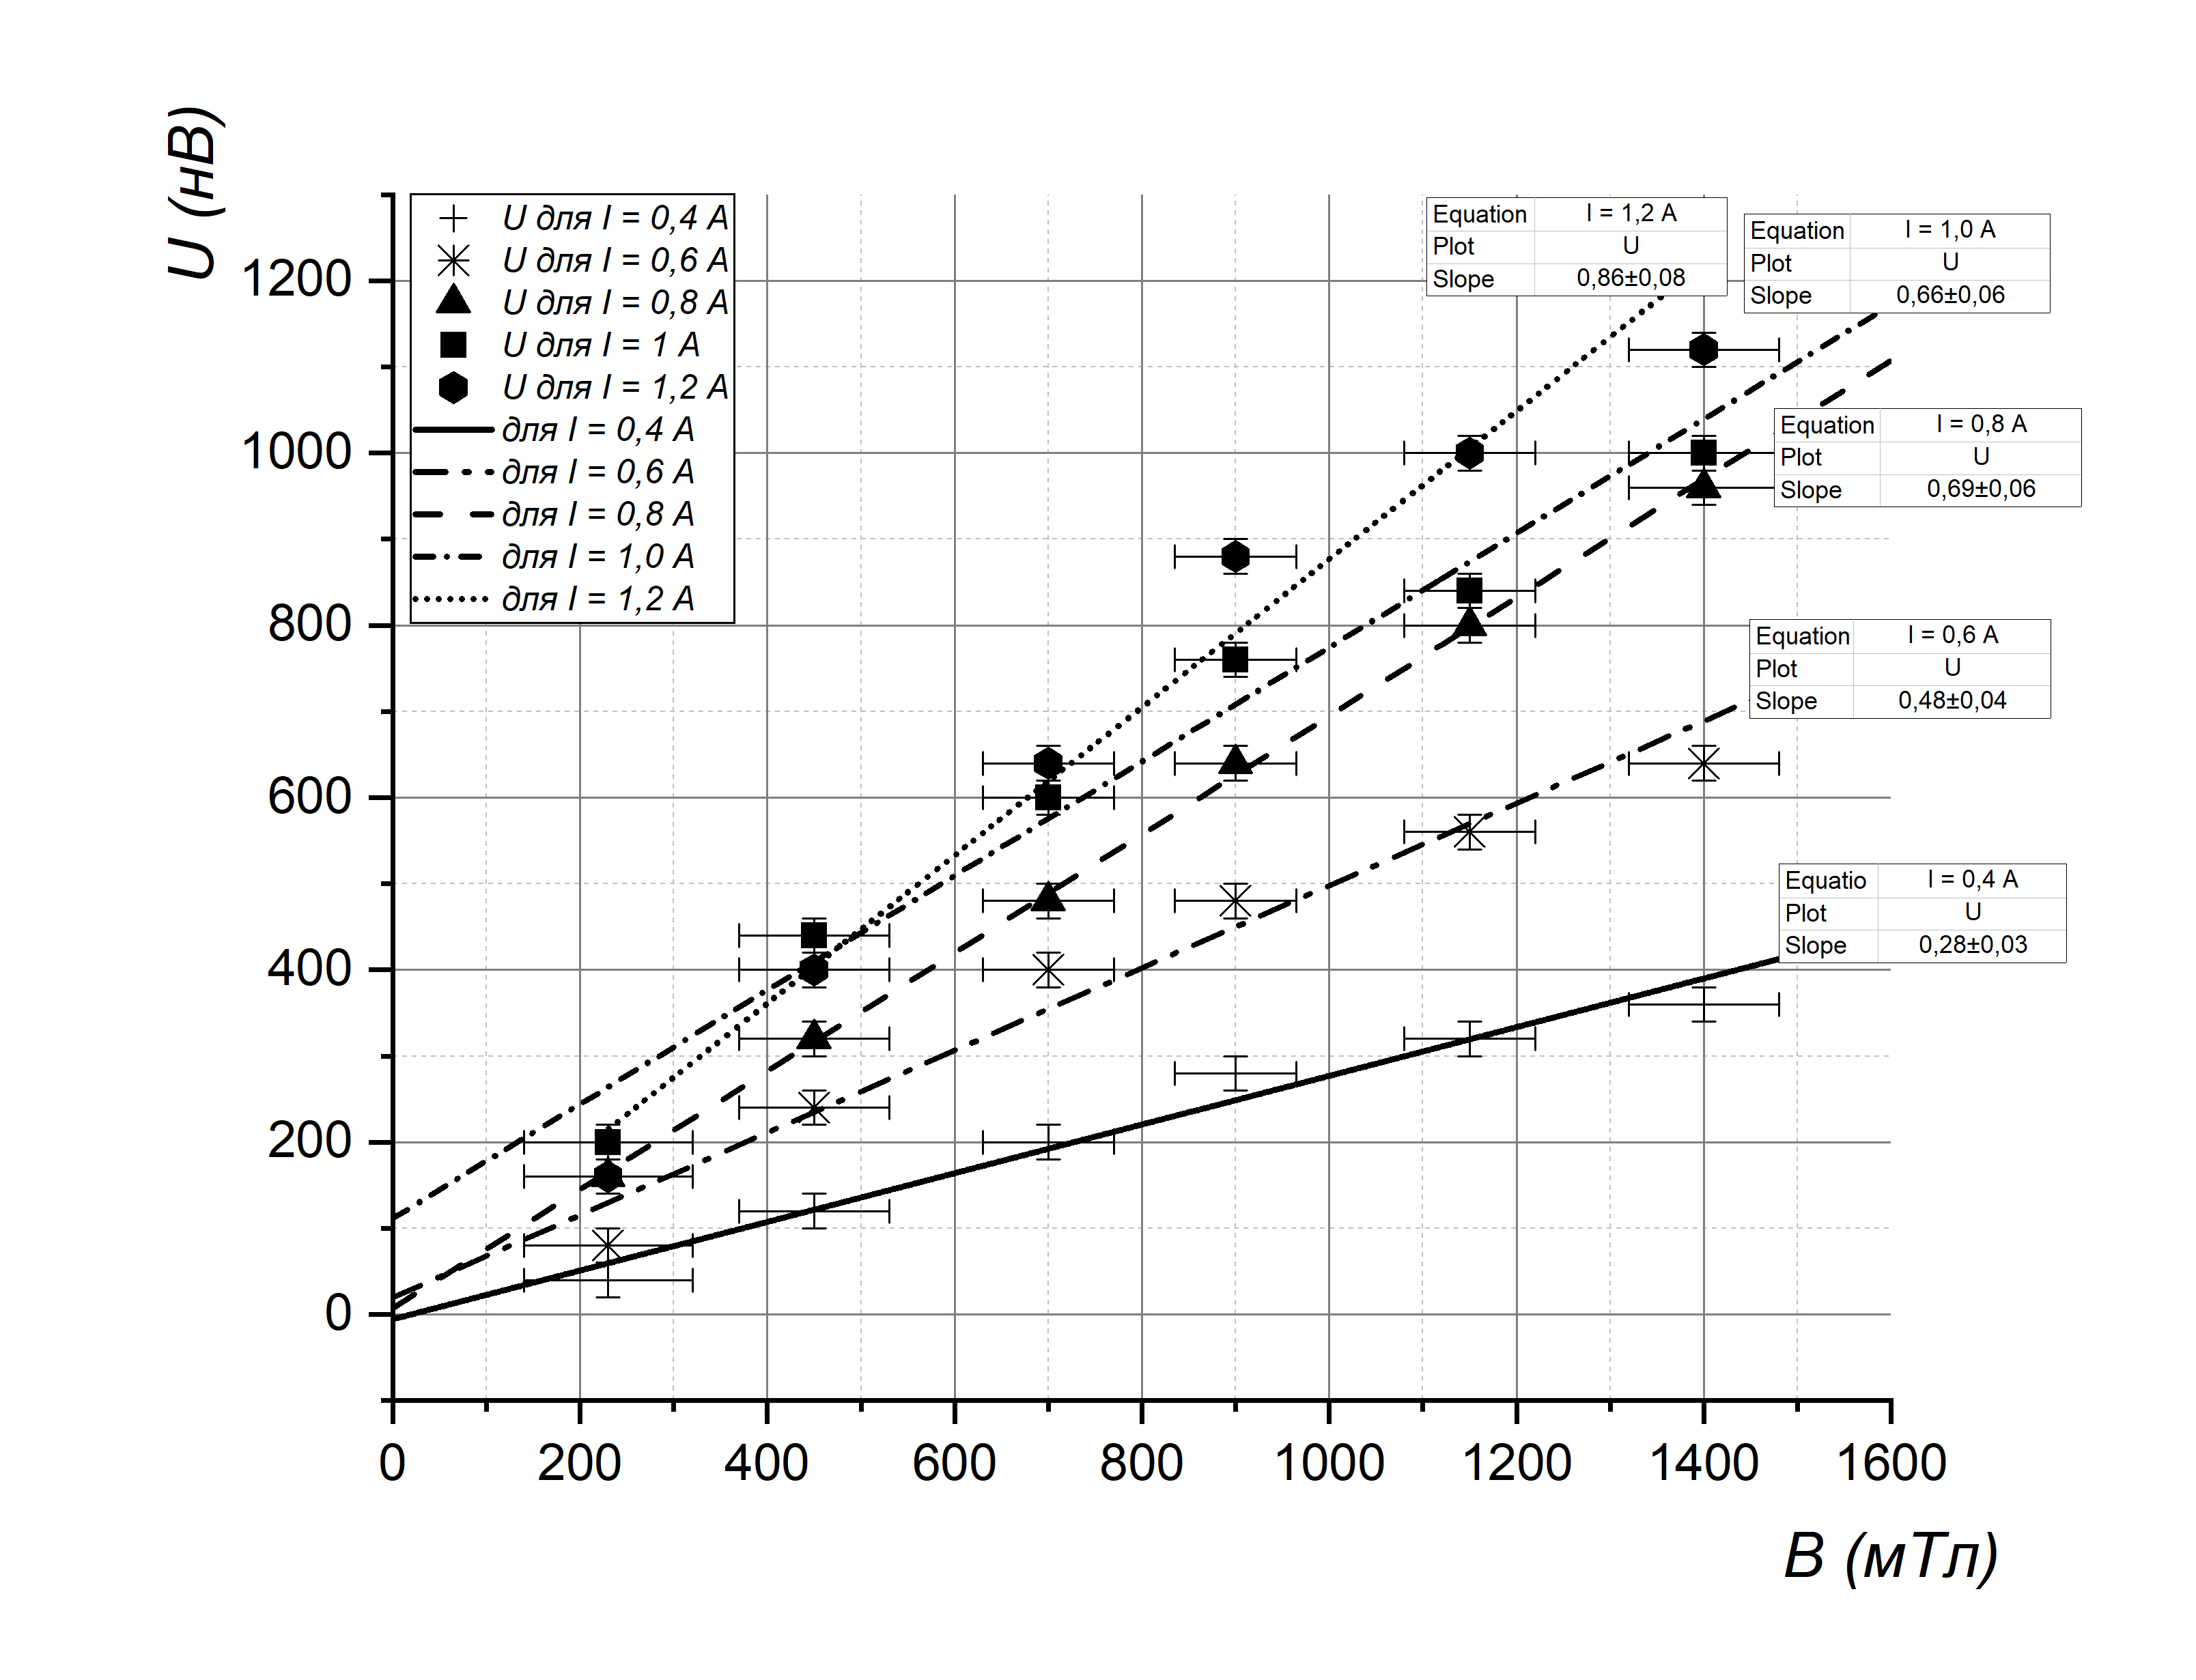
\includegraphics[width = \textwidth]{2.jpg}
\textbf{График 2.} Нахождение $\varepsilon_x = f(B)$
\end{center}
Далее находим функцию зависимости $k = f(I)$, где $k$ - коэффициент угла наклона для каждого из токов.\\
\begin{center}
\begin{tabular}{|c|c|c|c|c|}
\hline
 & $I$, A & $\sigma_{I}$, A & $k$, $\dfrac{\text{мкВ}}{\text{Тл}}$ & $\sigma_k$, $\dfrac{\text{мкВ}}{\text{Тл}}$ \\ \hline
1 & 0,4 & 0,01 & 0,28 & 0,03 \\ \hline
2 & 0,6 & 0,01 & 0,48 & 0,04 \\ \hline
3 & 0,8 & 0,01 & 0,69 & 0,06 \\ \hline
4 & 0,9 & 0,01 & 0,66 & 0,06 \\ \hline
5 & 1 & 0,01 & 0,86 & 0,08 \\ \hline
\end{tabular}\\
\textbf{Таблица 7:}Функция $k = f(I)$
\end{center}
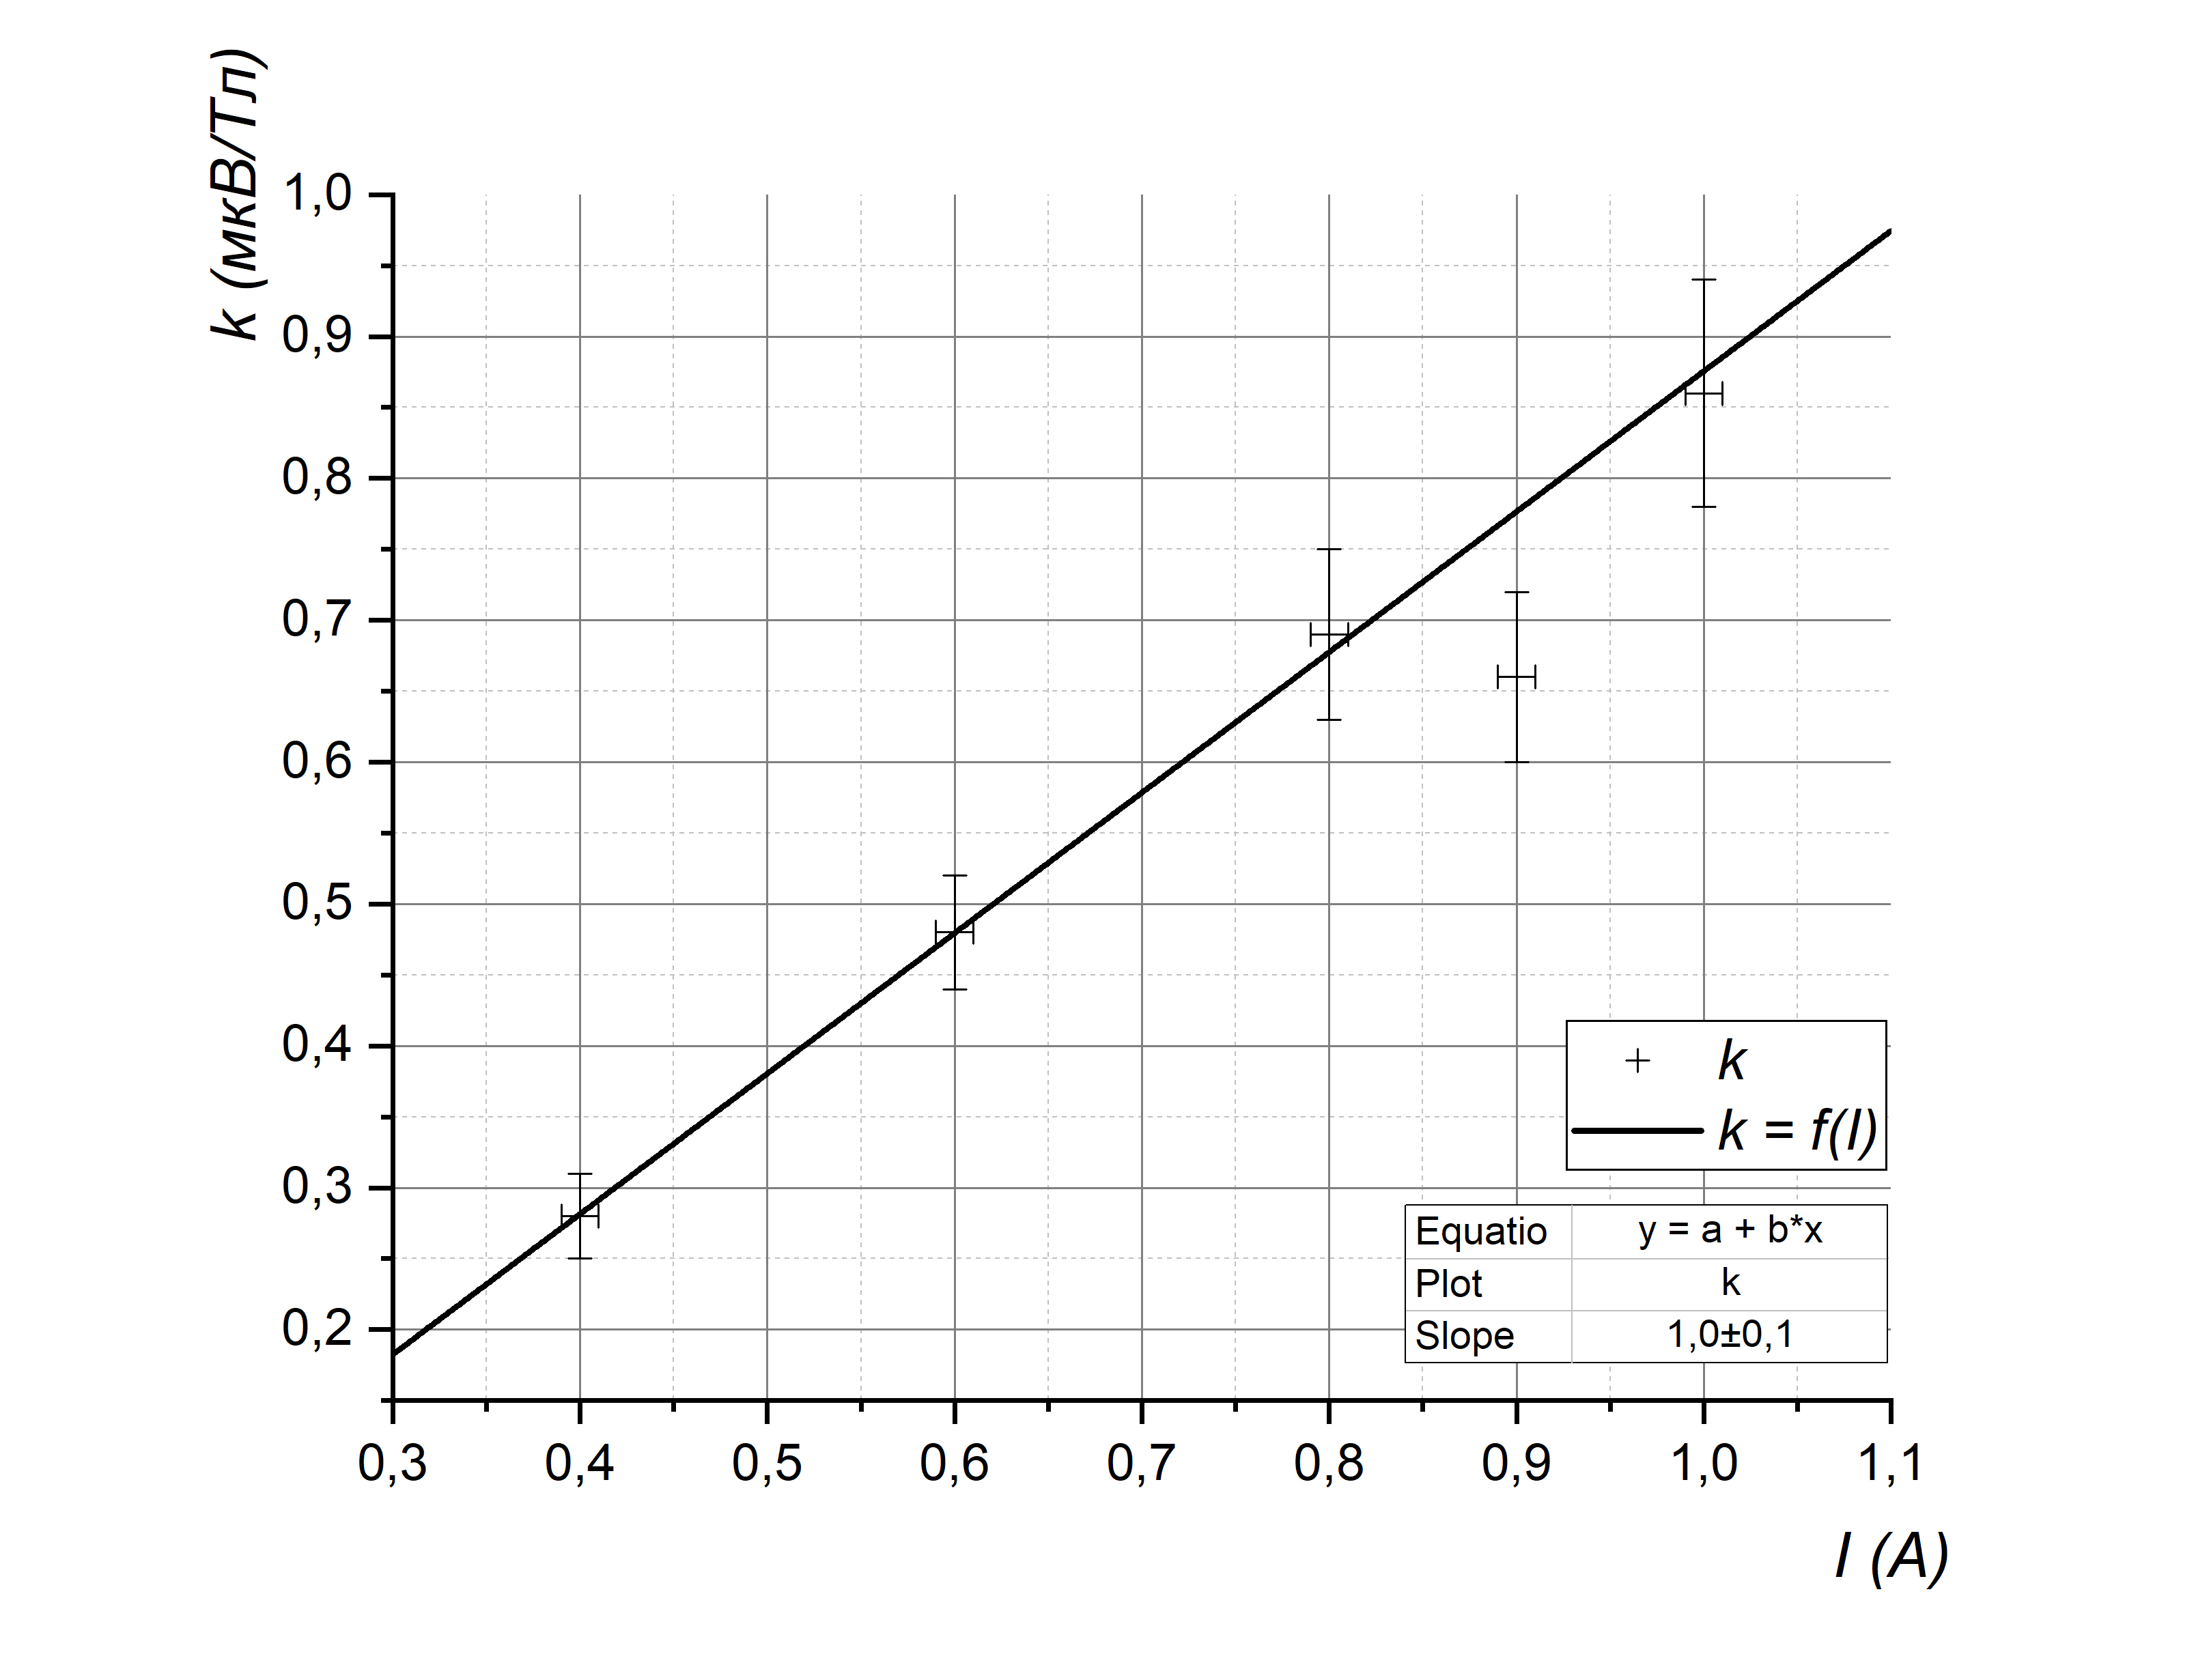
\includegraphics[width = \textwidth]{3.jpg}\\
\begin{center}
\textbf{График 3.} Нахождение $k = f(I)$
\end{center}
\begin{center}
\begin{tabular}{|c|c|c|}
\hline
 & Цинк & Медь \\ \hline
$L_{34}$, мм & 4 & 6 \\ \hline
$a$, мм & 0,08 & 0,05 \\ \hline
$l$, мм & 10 & 8 \\ \hline
$U_{34}$, мкВ & 26 & 23 \\ \hline 
\end{tabular}\\
\textbf{Таблица 8.} Некоторые характеристики образцов.
\end{center}
Из угла наклона графика зависимости $k = f(I)$ мы получаем, что угол наклона этого графика $A = (1,0 \pm 0,1) \dfrac{\text{мкОм}}{\text{Тл}}$\\
Из этого мы получаем, что из формулы (5) следует, что 
\[R_x = -A \cdot a = -(5 \pm 0,5) \cdot 10^{-11} \dfrac{\text{м}^3}{\text{Кл}}\]
Сравнивая с таблицей из лабораторного практикума по общей физике, удостовериваемся, что наше значение, в пределах ошибки, совпадает с табличным, равным $-5,3 \cdot 10^{-11} \dfrac{\text{м}^3}{\text{Кл}}$
\begin{center}
\begin{tabular}{|c|c|c|c|c|c|c|c|}
\hline
 & \multicolumn{3}{c|}{$I = 0,6$ A} & \multicolumn{4}{c|}{$U_0 = 10$ нВ} \\ \hline
 & $I_{\text{м}}$, А & $\sigma_{I_{\text{м}}}, A$ & $\sigma_B$, мТл & $B$, мТл & $U$, ед & $U$, нВ & $\sigma_{U}$, нВ \\ \hline
1 & 0,20 & 0,01 & 130 & 230 & 16 & 240 & 20 \\ \hline
2 & 0,40 & 0,01 & 80 & 450 & 22 & 480 & 20 \\ \hline
3 & 0,60 & 0,01 & 70 & 700 & 27 & 680 & 20 \\ \hline
4 & 0,80 & 0,01 & 65 & 900 & 30 & 800 & 20 \\ \hline
5 & 1,00 & 0,01 & 70 & 1150 & 33 & 920 & 20 \\ \hline
6 & 1,20 & 0,01 & 80 & 1400 & 36 & 1040 & 20 \\ \hline
\end{tabular}\\
\textbf{Таблица 9:}$\varepsilon_x = f(B)$ для цинка.
\end{center}
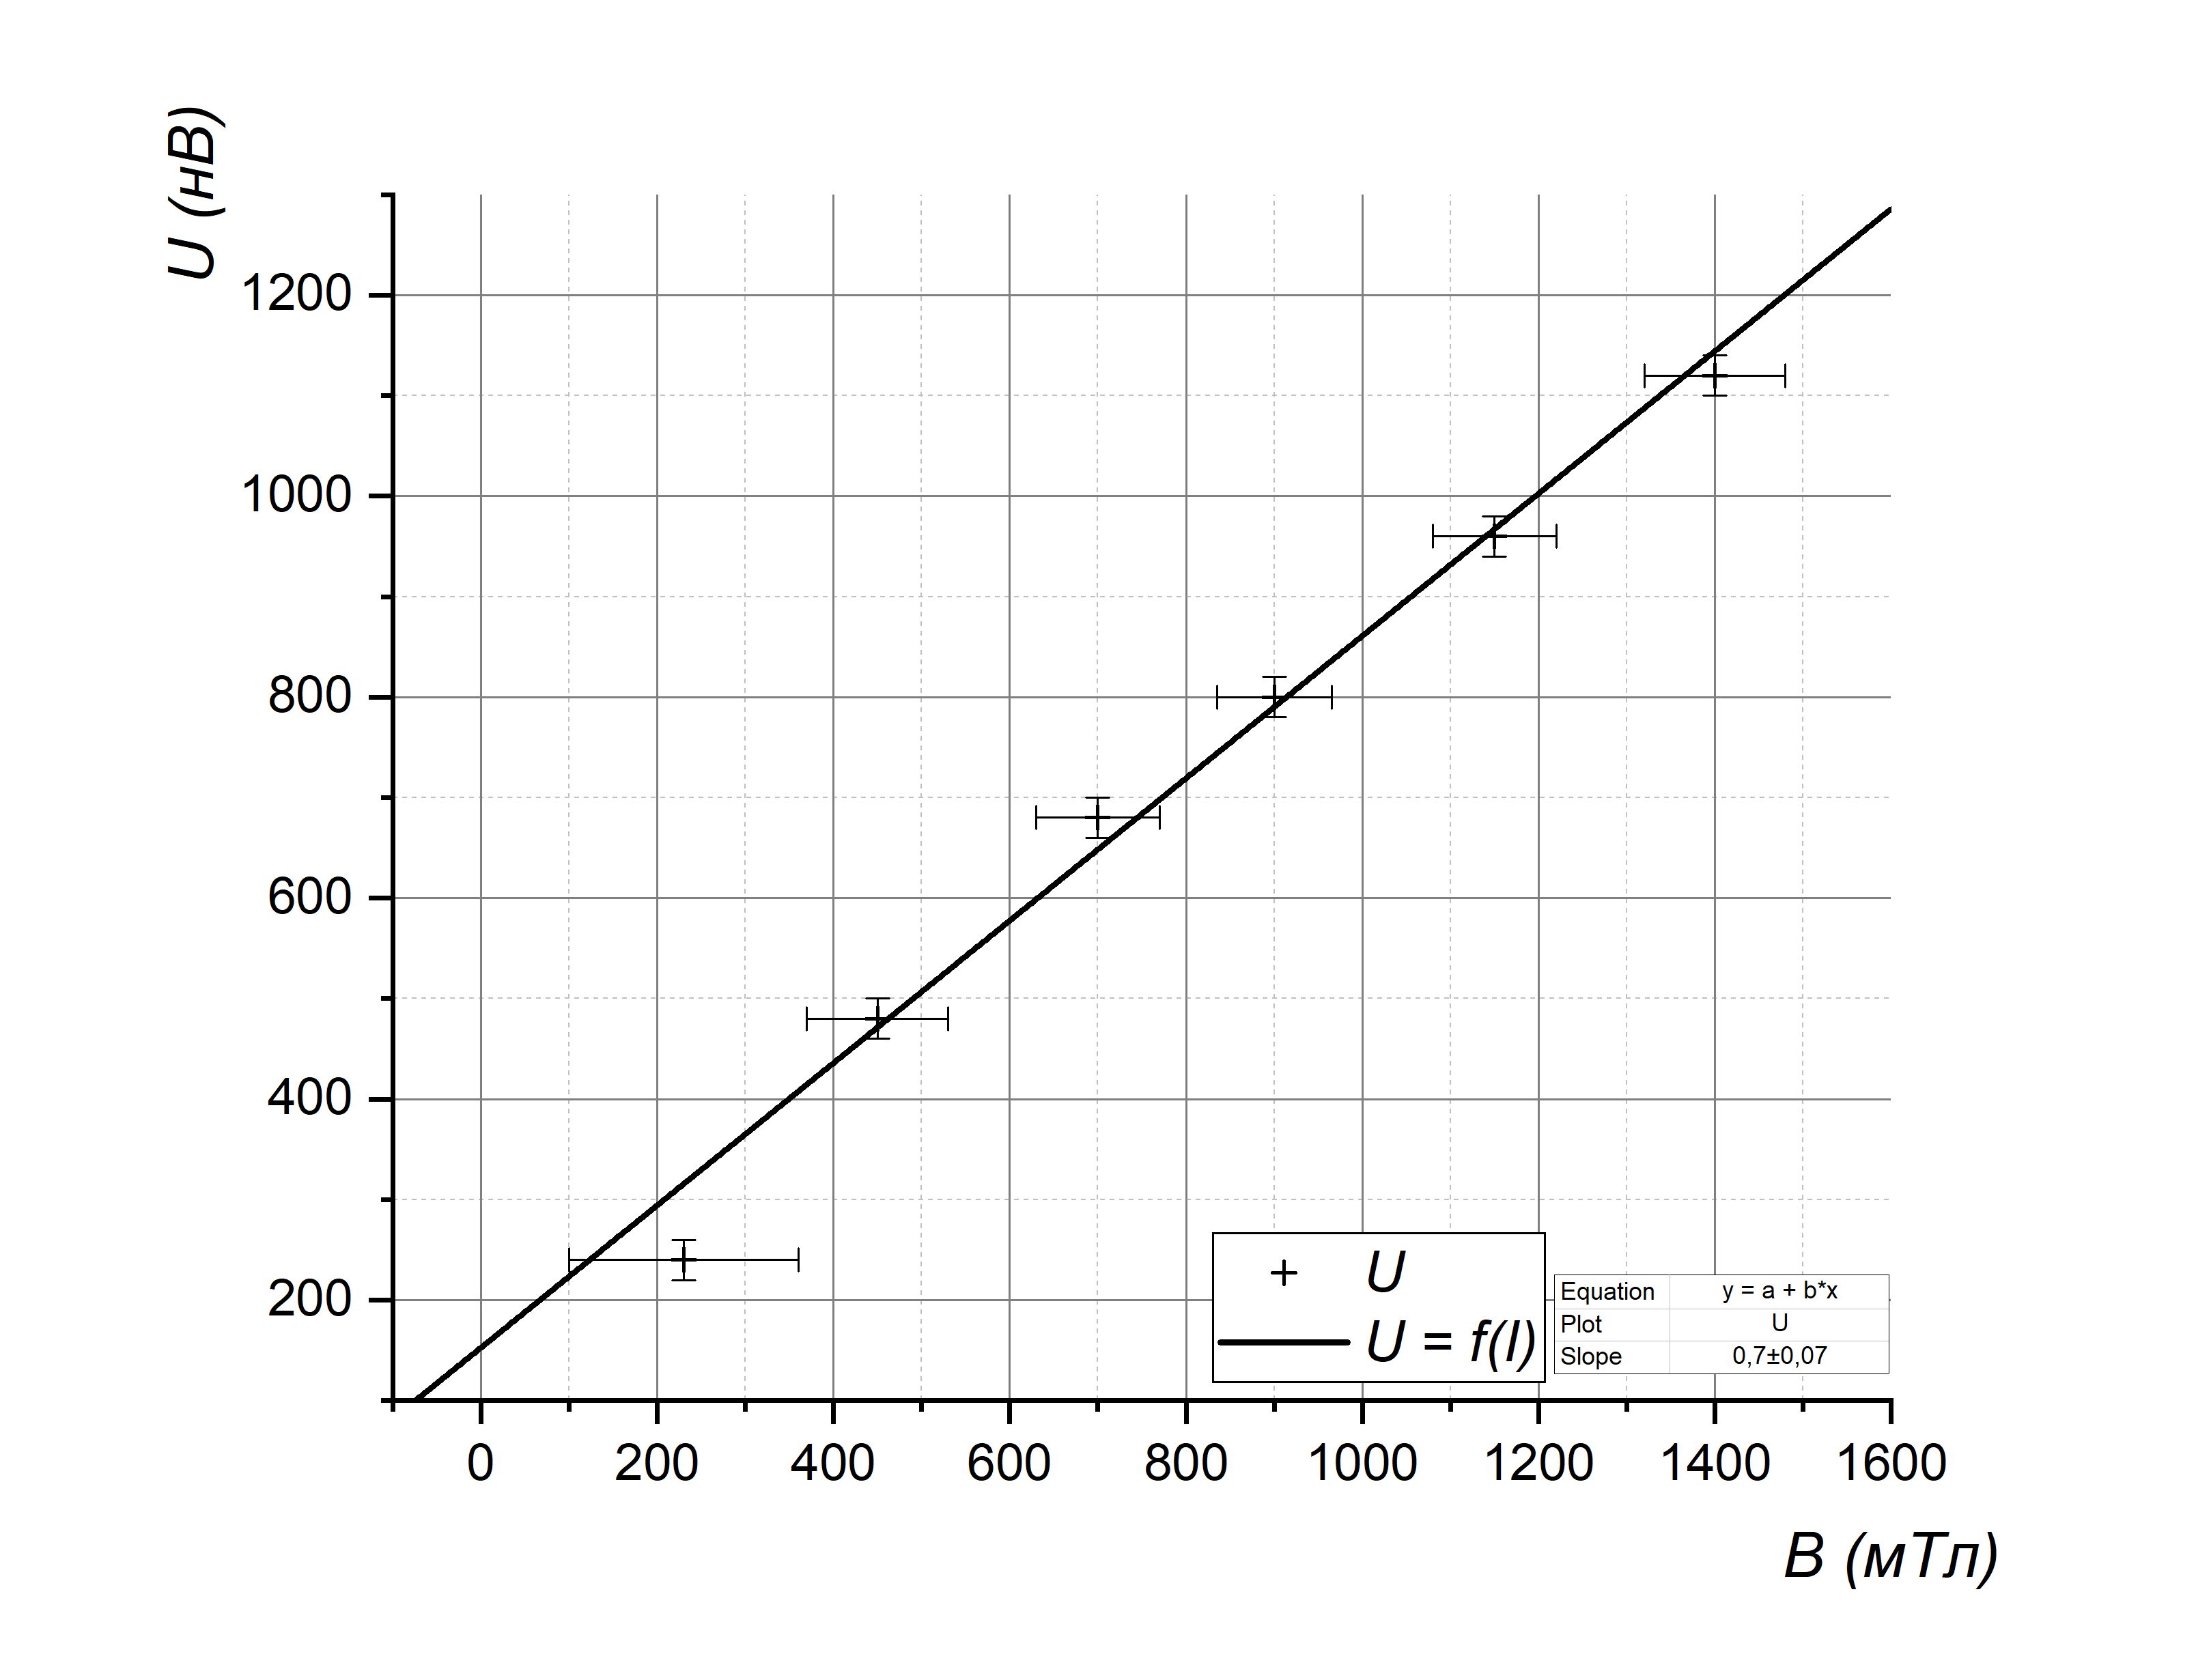
\includegraphics[width = \textwidth]{4.jpg}\\
\begin{center}
\textbf{График 4.} Нахождение $U = f(B)$ для цинка (ток течет в обратном направлении).
\end{center}
Теперь ищем то же самое для цинка: 
\[B = (0,7 \pm 0,07) \dfrac{\text{мкВ}}{\text{Тл}}\]
\[R_x = - \dfrac{B \cdot a}{I} = (9,5 \pm 0,9) \cdot 10^{-11} \dfrac{\text{м}^3}{\text{Кл}}\]
Сравнивая с табличным значением, взятым из той же таблицы, что и для меди, удостовериваемся, что наше значение, с учетом погрешности совпадает с табличным, равным $1,04 \cdot 10^{-11} \dfrac{\text{м}^3}{\text{Кл}}$\\
Далее рассчитаем концентрацию носителей тока по формуле (6)\\
Для меди: $ n = \dfrac{1}{R_x \cdot e} = -(0,12 \pm 0,01) \cdot 10^{30} \dfrac{1}{\text{м}^3}$\\
Для цинка: $n = (0,60 \pm 0,06) \cdot 10^{30} \dfrac{1}{\text{м}^3}$\\
Рассчитаем удельную проводимость $\sigma$ для образцов по формуле (7).\\
Для меди: $\sigma = (0,63 \pm 0,06) \cdot 10^8 \dfrac{1}{\text{Ом} \cdot \text{м}}$\\
Для цинка: $\sigma = (0,19 \pm 0,02)\cdot 10^8 \dfrac{1}{\text{Ом} \cdot \text{м}}$\\
Сверяя с табличными данными, получаем, что в пределах ошибки наши данные с ними совпадают($5,6 \cdot 10^7 \dfrac{1}{\text{Ом} \cdot \text{м}}$ для меди и $1,6 \cdot 10^7 \dfrac{1}{\text{Ом} \cdot \text{м}}$ для цинка)\\
Используя найденные значения рассчитываем подвижность носителей по формуле 
\[b = \dfrac{\sigma}{n \cdot e} = R_x \cdot \sigma\]
Для меди: $b = (32 \pm 3) \dfrac{\text{см}^2}{\text{В} \cdot c}$\\
Для цинка: $b = (18 \pm 2) \dfrac{\text{см}^2}{\text{В} \cdot c}$\\
Удостовериваемся, что наши данные в пределах ошибки совпадают с табличными ($32 \dfrac{\text{см}^2}{\text{В} \cdot c}$ для меди и $17,5 \dfrac{\text{см}^2}{\text{В} \cdot c}$ для цинка).
\section*{Используемая литература.}
\begin{enumerate}
\item \textbf{Лабораторный практикум по общей физике:} Учебное пособие. В трех томах. Т. 2. Электричество и магнетизм /Гладун А.Д., Александров Д.А., Берулёва Н.С. и др.; Под ред. А.Д. Гладуна - М.: МФТИ, 2007. - 280 с.
\item \textbf{Дополнительное описание лабораторной работы 3.3.5}: Эффект Холла в металлах; Под ред. МФТИ, 2016. - 5 с.
\end{enumerate}
\end{document}

